\documentclass{article}
\usepackage{xcolor}
\usepackage{graphicx}
\usepackage{float}
\usepackage{tikz}
\usepackage{parskip}
\usepackage{amsmath}
\usepackage{amsthm}
\usepackage{amssymb}
\usepackage{mathtools}
\usepackage{fancyhdr}
\usepackage[%paperheight = 59.4cm,
            %paperwidth = 42cm,
            %includehead,
            nomarginpar,
            textwidth=15cm,
            headheight=10mm]{geometry}


\begin{document}
 
\pagestyle{fancy}
%\fancyhead{}\fancyfoot{}

\fancyhf[OHC]{Christopher Munoz WRH2 Optimization}
\textbf{Problem 2.4:} \\
We are given the following expression and are tasked with graphing the feasible set and determining any local or global minimizers:
\begin{align*}
    \text{minimize} &\null \quad f(x) = x_1 \\
    \text{subject to} &\null \quad (x_1 - 1)^2 + x_2^2 = 1 \\ 
    &\null \quad (x_1+1)^2 + x_2^2 = 1
\end{align*}
Below is the graph of the feasible set:

\begin{figure}[H]
    \centering
    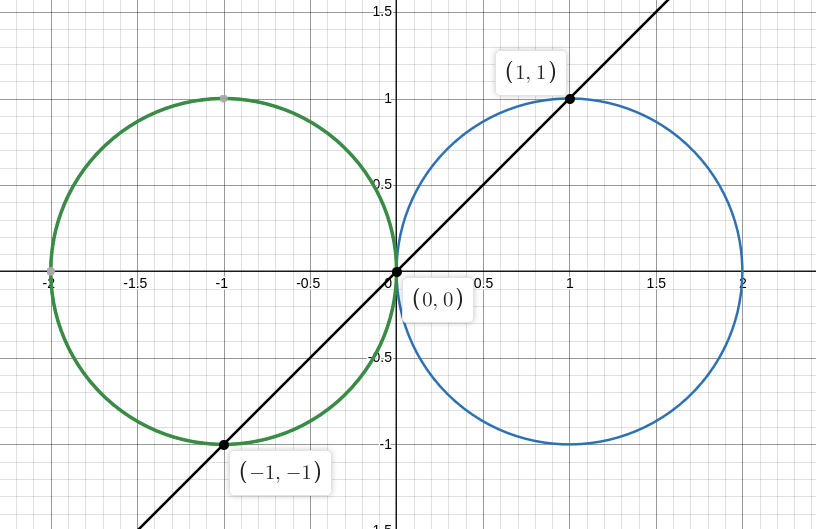
\includegraphics[scale = 0.40]{desmos1.png}
\end{figure}
Because our objective function is linear, the local minimizer and the global minimizer are the same value. We determine that (-1, -1) is both our global and local minimizer.
\break
\break
\textbf{Problem 2.5:} In this exercise we are tasked with providing an example function that nas no global minimizer and no global maximizer. If we take any linear function without constraints we will have no global minimizer or maximizer. The function $f(x) = x_1$ for example.
\break \break
\textbf{Problem 2.7:} \underline{Theorem:} Given $f(x)$ for $x \in S$ and $S$ is the set of all integers, Every point in $S$ is a local minimizer in $f$.
\newline
\underline{Proof:} First note that since $x \in S$, then $x-1$ and $x+1$ must also be in S.  Suppose x is a local minimizer, replacing x with the values of $x-1$ or $x+1$ should yield us values greater than $f(x)$. Then we know that $f(x) \leq f(x+1)$ and $f(x) \leq f(x-1)$ by definition of local minimizer. 
\break \break
\textbf{Problem 3.1:} \underline{Theorem:} The intersection of a finite number of convex sets is also a convex set.
\newline \underline{Proof:} Suppose $S$ is the intersection of a finite number of convex sets and $S \subseteq \mathbb{R}^n$. We will show that $S$ is also convex. Let $G_1, G_2, ... , G_n$ be convex sets where $G_1, G_2, ... , G_n = S$, let $x, y \in S$ and $\alpha \in [0,1]$. We want to show that $\alpha x + (1-\alpha)y \in S$, Since $x,y \in S$, then $x,y \in G_i$ for all $i$ in $ \{1, 2, ..., n\} $. This would mean that $\alpha x + (1 - x)y$ is in $G_i$ for all $i$ in $\{1,2,...,n\}$. Thus $\alpha x + (1 - x)y \in S$, therefore proving that the interesection of a finite number of convex sets is itself convex.
\break
\break
\textbf{Problem 3.3:} \underline{Theorem:} Given the feasible region S defined by a set of linear constraints
\begin{align*}
    S = \{ x : Ax \leq b \}
\end{align*}
$S$ is convex.
\newline \underline{Proof:} For a $S$ to be convex then $S$ must satisfy $x,y \in S$ and $\alpha x + (1 - \alpha) \in S$ where $\alpha \in [0,1]$, also $S$ is a subset of $\mathbb{R}^n$.  Suppose $Ax \leq b$ and $Ay \leq b$, we consider the following:
\begin{align*}
    A(\alpha x + (1 - \alpha)y) & = A\alpha x + (1 - \alpha)Ay \\
    & \leq \alpha b + (1 - \alpha)b \\
    & \leq \alpha b + b - \alpha b \\
    & \leq b 
\end{align*}
This shows that our region S defined by a set of set of linear constraints $S = \{ x : Ax \leq b \}$ is convex. $\blacksquare$
\break
\break
\textbf{Problem 3.7:} \underline{Theorem:} Let $f$ be a convex function on a convex set $S \in \mathbb{R}^n$. Let $k$ be a nonzero scalar and define $g(x) = kf(x)$, we also let $x,y \in \mathbb{R}$ and $\alpha \in [0,1]$. If  $k > 0$, then $g$ is a concave function on set $S$, if $k < 0$, then $g$ is a concave function on set $S$.
\newline \underline{Proof for $k > 0$:} We start with the case of $k > 0$, in order to show convexity we need to show that $g(\alpha x + (1 - \alpha)y)  \leq \alpha g(x) + (1 - \alpha)g(y)$. Substituting $g(x)$ with $kf(x)$ we consider the following using the definition of convexity:
\begin{align*}
    kf(\alpha x + (1 - \alpha)y) & \leq \alpha kf(x) + (1 - \alpha)kf(y) \\ 
    & \leq k(\alpha f(x) + (1 - \alpha)f(y)) 
\end{align*}
Since $k > 0$ we can divide both sides by k and retain signage giving us
\begin{align*} 
    f(\alpha x + (1 - \alpha)y) \leq \alpha f(x) + (1 - \alpha)f(y)
\end{align*}
Which is the very definition of convexity. \newline
\underline{Proof for $k < 0$:} Lets suppose $k < 0$, we can show cocavity with the following, note that since k is negative we flip the sign:
\begin{align*}
    kf(\alpha x + (1 - \alpha)y) & \geq \alpha kf(x) + (1 - \alpha)kf(y) \\
    & \geq k(\alpha f(x) + (1 - \alpha)f(y)) \\
    & \geq \alpha f(x) + (1 - \alpha)f(y)
\end{align*}
Thus showing that when $k > 0$, $g$ is convex and when $k < 0$, $g$ concave. $\blacksquare$
\break
\break
\textbf{Problem 3.13:} \underline{Theorem:} If $f$ is a convex function on the convex set $S$ then the level set
\begin{align*}
    T = \{ x \in S : f(x) \leq k \}
\end{align*}
is convex for all real number $k$. \newline
\underline{Proof:} Let there be an $x,y \in S$ such that $f(x) \leq k$, $f(y) \leq k$ and $\alpha \in [0,1]$ We begin with out convexity definition:
\begin{align*}
    f(\alpha x + (1 - \alpha)y) & \leq \alpha f(x) + (1 - \alpha)f(y) \\
    & \leq \alpha k + (1 - \alpha)k \\
    & \leq \alpha k + k - \alpha k \\
    & \leq k
\end{align*}
This is sufficient in showing convexity. $\blacksquare$
\newline
\break
\textbf{Problem 3.18:} $(2,2)^T$ can be expressed as a convex combination of $(0, 0)^T$, $(1,4)^T$ and $(3,1)^T$, \\
What we ultimately mean to solve for the coefficients of the system of equations:
\begin{align*}
    \lambda_1(0) + \lambda_2(1) + \lambda_3(3) = 2 \\
    \lambda_1(0) + \lambda_2(4) + \lambda_3(1) = 2
\end{align*}
We solve below:
\begin{align}
    \begin{bmatrix}
        0 & 1 & 3 \\
        0 & 4 & 1
    \end{bmatrix}
    = (2,2)^T & \Rightarrow 
    \begin{bmatrix}
        0 & 1 & 3 & 2 \\
        0 & 4 & 1 & 2   
    \end{bmatrix} \\ 
    & \Rightarrow
    \begin{bmatrix}
        0 & 1 & 3 & 2 \\
        0 & 0 & -11 & -6 
    \end{bmatrix} & \text{multiply top row by -4, add to bottom row } \\ & \Rightarrow
    \begin{bmatrix}
        0 & 1 & 3 & 2 \\
        0 & 0 & 1 & 6/11
    \end{bmatrix} & \text{divide bottom row by -11}
\end{align}
We plug $6/11$ into the top row of our matrix $(3)$ and we get $(2,2)^T = n(0, 0)^T + \frac{4}{11}(1,4)^T + \frac{6}{11}(3,1)^T$
for any $n \in \mathbb{R}$.
\newline
\break
\textbf{Problem P5:} For the following functions we determine if the function is convex, concave, both or neither, for the following functions we let $x,y \in \mathbb{R}$ and $\alpha \in [0,1]$ and we use the definition of convexity $f(\alpha x + (1 - \alpha)y) \leq \alpha f(x) + (1 - \alpha)f(y)$ and concavity: $f(\alpha x + (1 - \alpha)y) \geq \alpha f(x) + (1 - \alpha)f(y)$.
\newline
\break
(a) - \underline{$f(x) = 9x - 14$} \qquad First we evaluate $f(\alpha x + (1 - \alpha)y) = 9(\alpha x + (1 - \alpha)y) - 14  \\ = 9 \alpha x + 9y - 9 \alpha y - 14$ and substitute for our lefthand side, we then evaluate the righthand side. 
\begin{align*}
    9 \alpha x + 9y - 9 \alpha y - 14 & \leq \alpha f(x) + (1 - \alpha)f(y) \\
    & \leq \alpha (9x-14) + (1 - \alpha)(9y-14) \\
    & \leq \alpha (9x-14) + (9y - 9y \alpha - 14 + 14 \alpha) \\
    & \leq 9x \alpha - 14 \alpha + 9y - 9y \alpha - 14 + 14 \alpha \\
    & \leq 9x \alpha + 9y - 9 \alpha y - 14
\end{align*}
As it turns out the left hand side is equal to the right hand side meaning that f(x) is convex, incidentally if we flip the sign the inequality would still be true, thus f(x) is both concave and convex. $\blacksquare$
\newline
\break
(b) - \underline{$f(x) = (1/3+x^4)$} \qquad For this one we'll just derive twice, we will use the second derivative definition and confirm positivity for all $x \in \mathbb{R}$.
\begin{align*}
    f(x) = \frac{1}{3} + x^4 \\
    f'(x) = 4x^3 \\
    f''(x) = 12x^2
\end{align*}
For all $x \in \mathbb{R}$, $f''(x)$ is positive, thus the function is strictly convex. $\blacksquare$
\newline
\break
(c) - \underline{$f(x) = \sqrt{1+x^2}$} \qquad For this function we determine using a second derivative test as well, we confirm positivity for all $x \in \mathbb{R}$.
\begin{align*}
    f(x) = \sqrt{1 + x^2} \\ 
    f'(x) = \frac{x}{\sqrt{1+x^2}} \\
    f''(x) = \frac{1}{(1+x^2)^\frac{3}{2}}
\end{align*}
For all $x \in \mathbb{R}$, $f''(x)$ is positive, the function is strictly convex. $\blacksquare$
\newline
\break
(d) - \underline{$f(x) = |x|$} \qquad The absolute value function can be expressed with the following piecewise function:
\begin{align*}
    f(x) = 
    \begin{cases}
        x & : 0 \leq x < \infty \\
        -x & : - \infty < x < 0 
    \end{cases}
\end{align*}
Suppose $x > 0$ and $y < 0$, we consider two cases, $\alpha x + (1 - \alpha)y > 0$ and $\alpha x + (1 - \alpha)y < 0$, we note that because it is an absolute value function, that $f(\alpha x + (1 - \alpha)y) = \alpha x + (1 - \alpha)y$
\newline Case 1: $\alpha x + (1 - \alpha)y > 0$
\begin{align*}
    f(\alpha x + (1 - \alpha)y) & = \alpha x + (1 - \alpha)y \\
    & = \alpha f(\alpha) - (1 - \alpha)f(y) 
\end{align*}
We note that $ \alpha f(\alpha) - (1 - \alpha)f(y) \leq \alpha f(x) + (1 - \alpha)f(y)$, meaning
\begin{align*}
 f(\alpha x + (1 - \alpha)y) \leq \alpha f(x) + (1 - \alpha)f(y)
\end{align*}
The very definition of convexity, proving the first case.
\newline
Case 2: $\alpha x + (1 - \alpha)y < 0$ \newline
Note:
\begin{align*}
    f(\alpha x + (1 - \alpha)y) & = -(\alpha x + (1 - \alpha)y) \\
    & = - \alpha x - (1 - \alpha)y \\
    & = - \alpha f(x) + (1 - \alpha)f(y)
\end{align*}
We note that $- \alpha f(x) + (1 - \alpha)f(y) \leq (1 - \alpha)f(y)$, therefore,
\begin{align*} 
    - \alpha f(x) + (1 - \alpha)f(y) & \leq \alpha f(x) + (1 - \alpha)f(y) \\
    & \text{thus} \\
    f(\alpha x + (1 - \alpha)y) & \leq \alpha f(x) + (1 - \alpha)f(y)
\end{align*}
The definition of convexity, proving case 2, the function $f(x)$ is convex. $\blacksquare$

\end{document}
